В этом эссе рассмотрим добавление frozen noise в различные системы.
 % при разной температуре и разной размерности. 
В частности убедимся в возникновение двух противоположных эффектов: \textit{термолизации} (иногда возникающей при небольшом уровне шума) и \textit{локализации} (при <<достаточном>> уровне шума). 

\red{Отлельный сюжет -- рост запутанности подсистем. Построить мостик со статьей, поговорить про $\tr \rho^2$ для подсистемы. Посмотреть на термальность матрицы плотности подсистемы.}

% Для полноты изложения и формирования первичной интуиции начнём с одночастичной задачи и андерсоновской локализации. 

Наличие шума приводит к неинтегрируемости системы, и иногда в этой изолированной квантовой системе в некотором смысле возникает термолизация. 
Что значит интерируемая квантовая система? Что такое \textit{термолизация}? Что такое \textit{ETH}?
Что такое \textit{локализация}? 
И к любому эффекту возникает вопрос какими метриками мы можем его охарактеризовать? Являются ли они достаточными и необходимыми? В чём принципиальное отличие MBL от Андерсоновской локализации?
\red{Хочется определить основные понятия, продемонстривовать как это всё работает. Потом в дополнение можно прокомментировать отдельные графики из статей} 


	
Рассмотрим one-dimensional Fermi-Hubbard model with 
\begin{equation*}
	\hat{H} = 
	- J \sum_{\langle i,j\rangle} (\hat{a}_i\D \hat{a}_j + \hc) 
	+ \Delta \sum_j \varepsilon_j \hat{n}_j
	+ V \sum_{\langle i,j\rangle} \hat{n}_i \hat{n}_j,
\end{equation*}
with равномерно-случайными $\varepsilon_j \in [-1,1]$. Эта система удобна тем, что можем посмотреть на различные экспериментальные реализации и в ней реализуются все интересные нам режимы. Я не буду здесь лезть в интегрируемые квантовые системы, и так хватает открытых вопросов. 



% Our main observable is the imbalance $I$ between the respective atom numbers on even ($N_e$) and odd ($N_o$) sites
% \begin{equation*}
% 	I = \frac{N_e - N_o}{}
% \end{equation*}

% J=1,V=0.5




\begin{figure}[h]
    \centering
    % 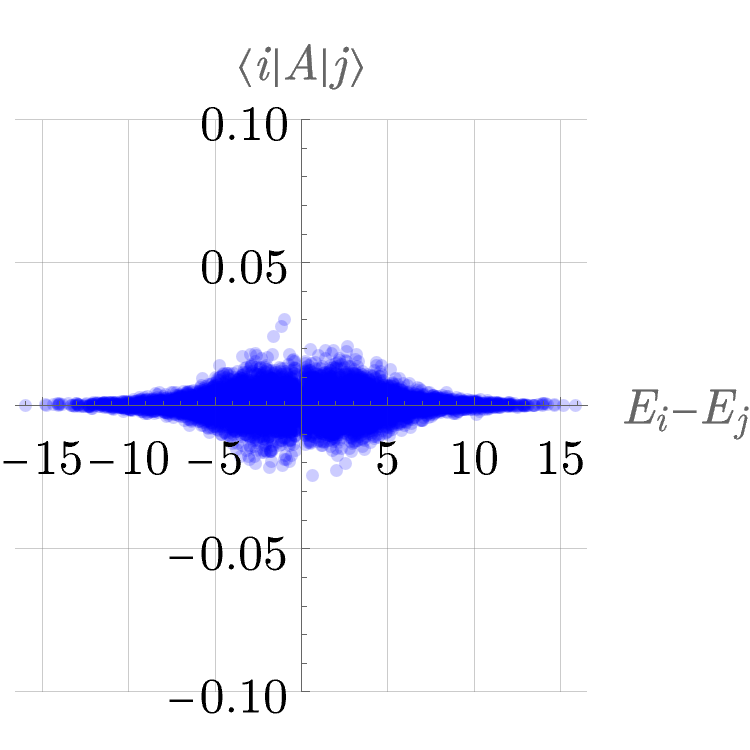
\includegraphics[align=c, width=0.25\textwidth]{imgs/lo1.png}
    \hspace{10 mm} 
    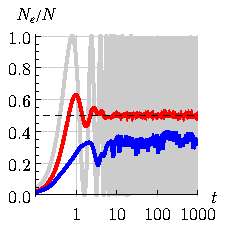
\includegraphics[align=c]{imgs/lo2.pdf}
    \hspace{1 mm} 
    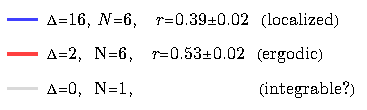
\includegraphics[align=c]{imgs/lo2l.pdf}
    \caption{labore et dolore magna aliquat enim ad minim veniam with $L=12$}
    %\label{fig:}
\end{figure}

Lorem ipsum dolor sit amet, consectetur adipisicing elit, sed do eiusmod
tempor incididunt ut labore et dolore magna aliqua. Ut enim ad minim veniam,
quis nostrud exercitation ullamco laboris nisi ut aliquip ex ea commodo
consequat. Duis aute irure dolor in reprehenderit in voluptate velit esse
cillum dolore eu fugiat nulla pariatur. Excepteur sint occaecat cupidatat non
proident, sunt in culpa qui officia deserunt mollit anim id est laborum.



\begin{figure}[h]
    \centering
    \addletter{45}{a}
    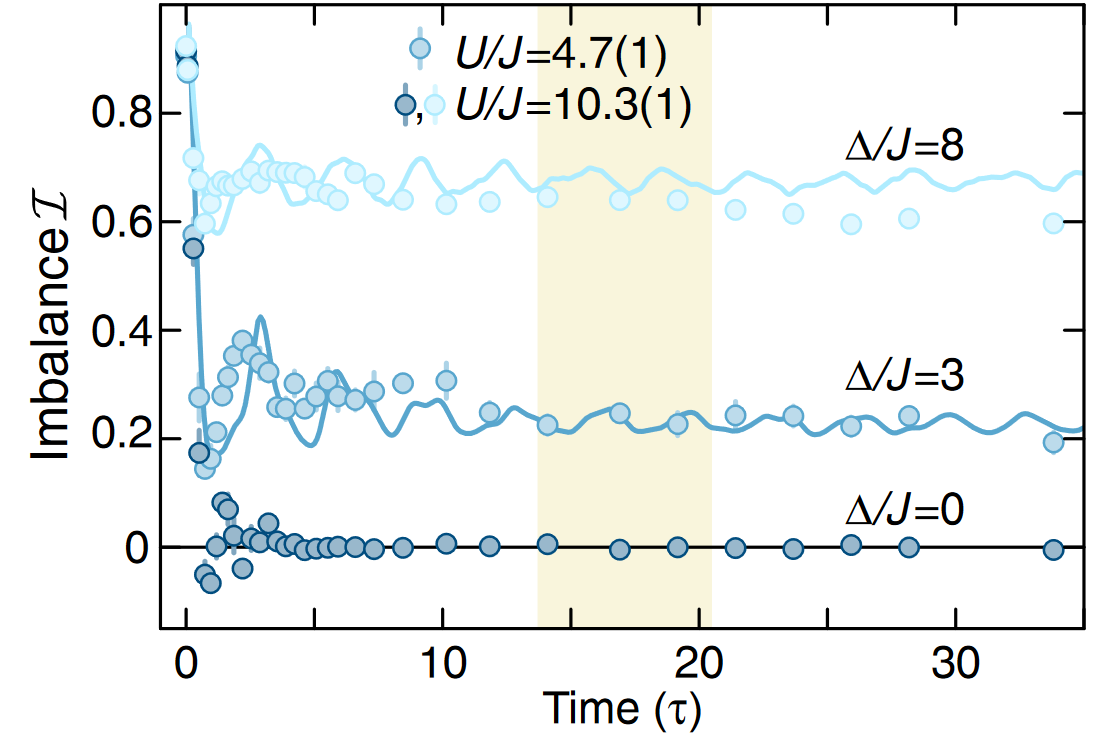
\includegraphics[align=c, width=0.35\textwidth]{imgs/MBL_exp_1.png}
    \hspace{10 mm} 
    \addletter{45}{b}
    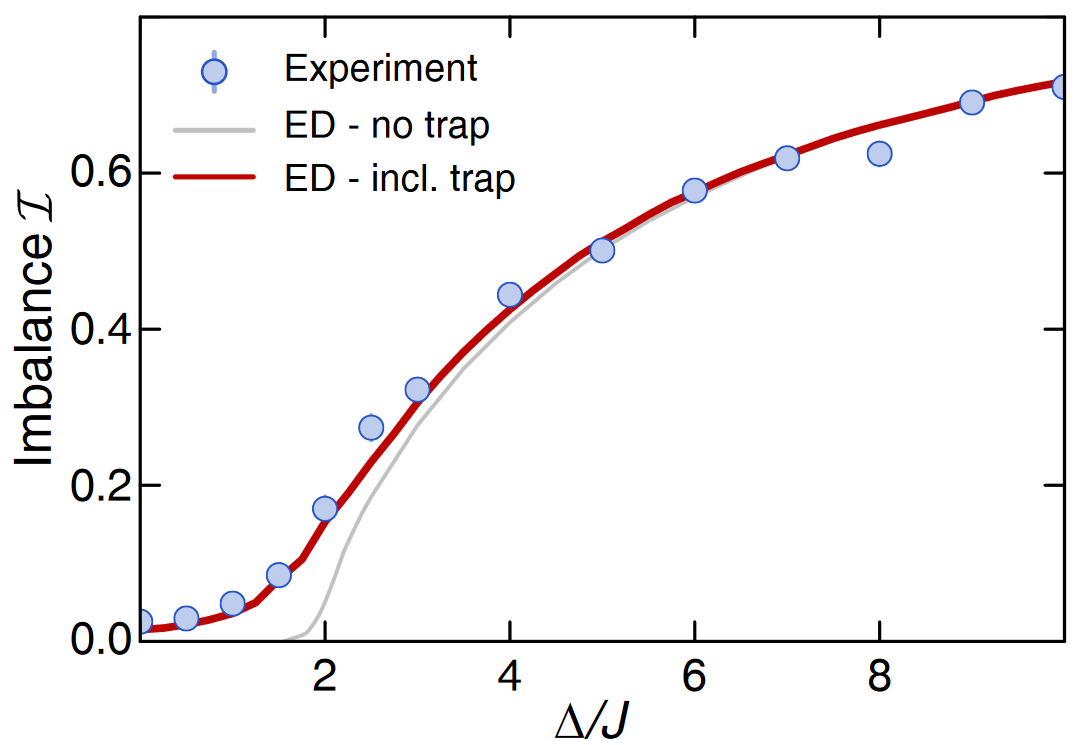
\includegraphics[align=c, width=0.35\textwidth]{imgs/MBL_exp_2.png}
    \caption{a) Time evolution of an initial charge-density wave. b) Stationary values of the imbalance $\mathcal{I}$ as a function of disorder $\Delta$ for non-interacting atoms \red{Основной вывод от этой картинки и этой статьи: есть локализация и термолизация. Взаимодействие влияет, но не столь принципиально.}}
    %\label{fig:}
\end{figure}



\newpage




Lorem ipsum dolor sit amet, consectetur adipisicing elit, sed do eiusmod
tempor incididunt ut labore et dolore magna aliqua. Ut enim ad minim veniam,

\begin{figure}[h]
    \centering
    \addletter{80}{a}
    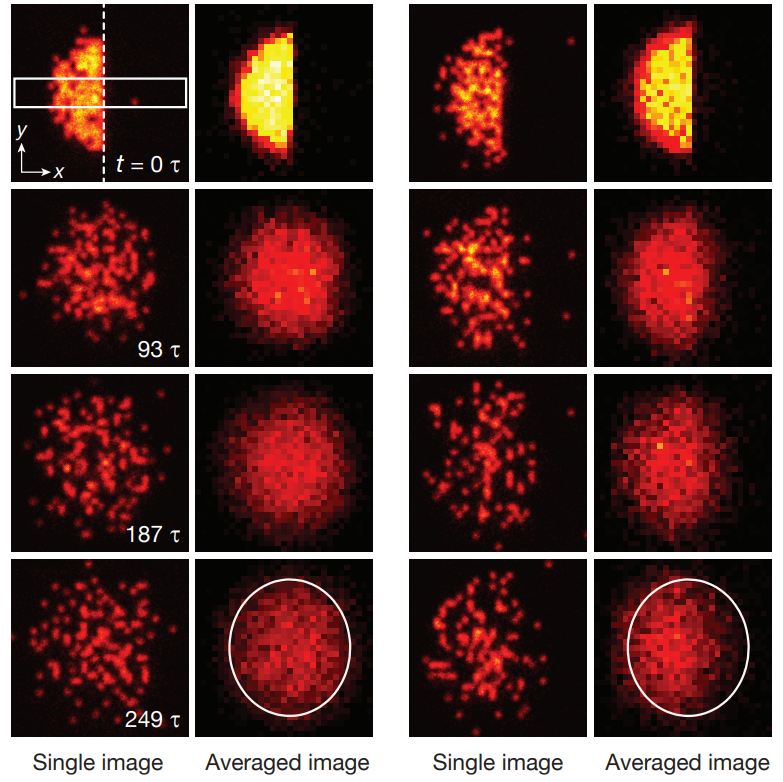
\includegraphics[align=c, width=0.33\textwidth]{imgs/MBL_2D_exp_1.png}
    \hspace{10 mm} 
    \addletter{80}{b}
    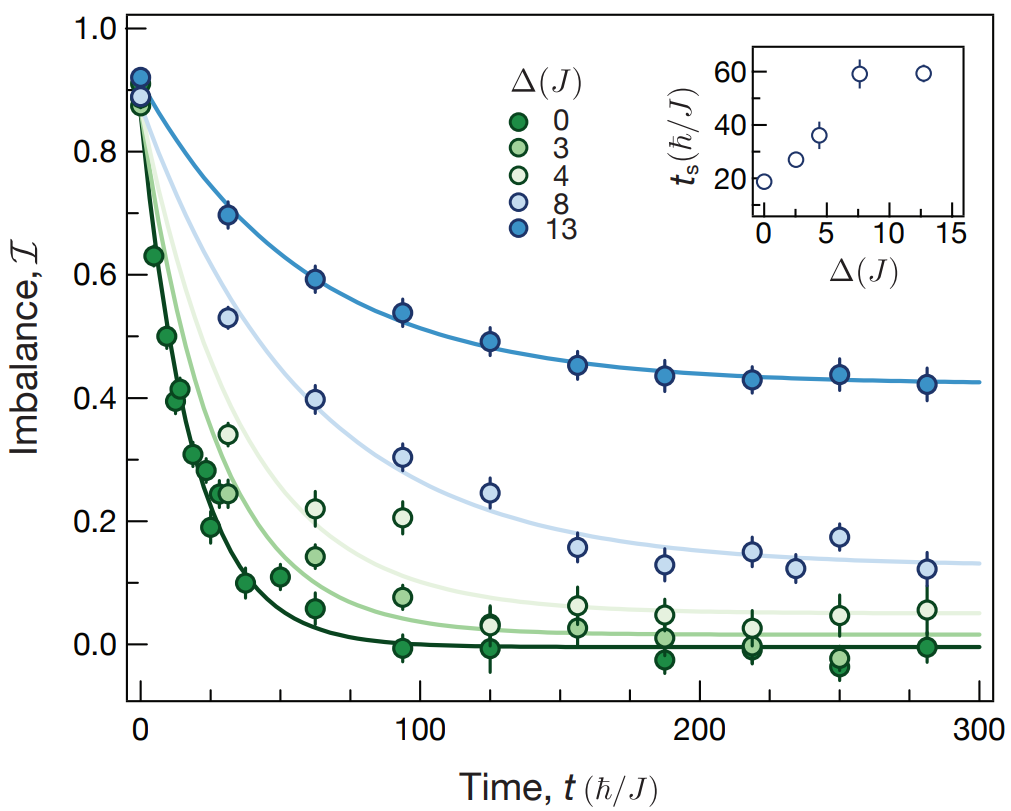
\includegraphics[align=c, width=0.4\textwidth]{imgs/MBL_2D_exp_2.png}
    % 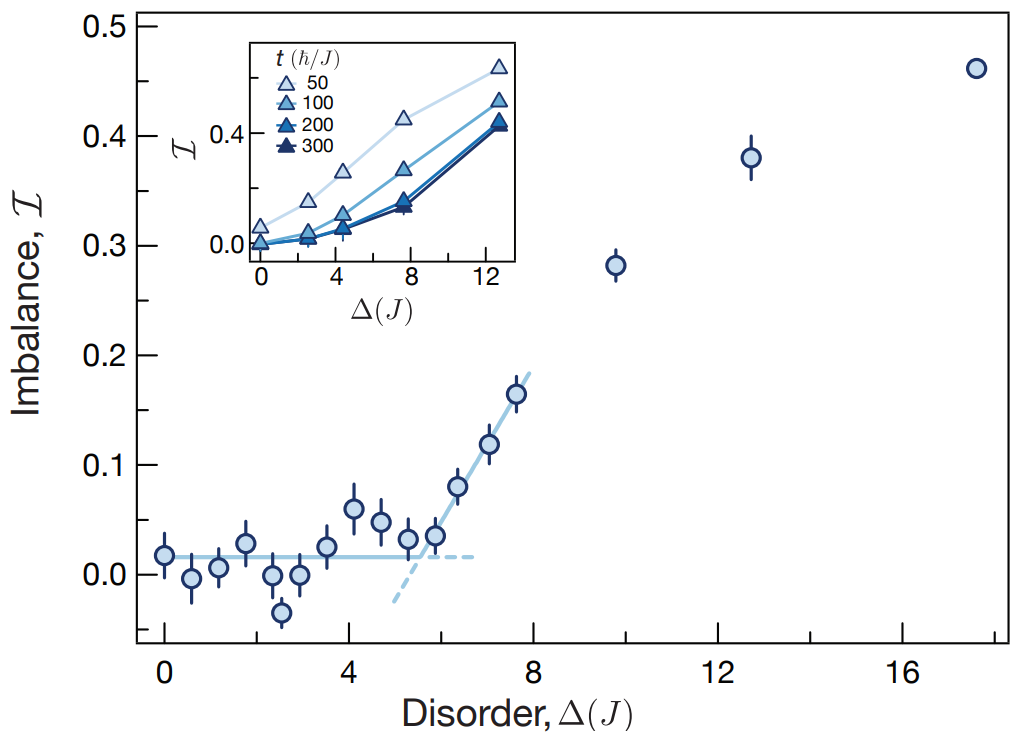
\includegraphics[align=c, width=0.4\textwidth]{imgs/MBL_2D_exp_3.png}
    \caption{
	    a) Raw fluorescence images (red to yellow corresponds to increasing detected light level) showing the evolution of the initial density step without disorder. 
	    b) Relaxation dynamics of a density domain wall.
    }
    %\label{fig:}
\end{figure}


Lorem ipsum dolor sit amet, consectetur adipisicing elit, sed do eiusmod
tempor incididunt ut labore et dolore magna aliqua. Ut enim ad minim veniam,
quis nostrud exercitation ullamco laboris nisi ut aliquip ex ea commodo
consequat. 

\begin{figure}[h]
    \centering
    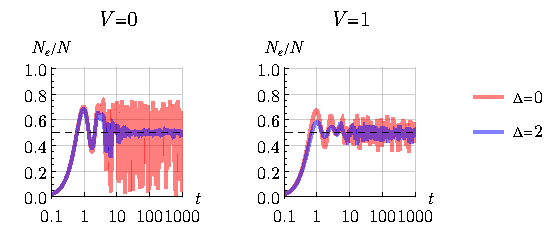
\includegraphics{imgs/loVD.pdf}
    \caption{$L=12$}
    %\label{fig:}
\end{figure}



Посчитать для зависимость $N_e/ N$ и $r$ от чего-нибудь. Добавить про map между Гейзенбергом и Хаббардом. 

\newpage

Lorem ipsum dolor sit amet, consectetur adipisicing elit, sed do eiusmod
tempor incididunt ut labore et dolore magna aliqua. Ut enim ad minim veniam,
quis nostrud exercitation ullamco laboris nisi ut aliquip ex ea commodo
consequat. Duis aute irure dolor in reprehenderit in voluptate velit esse
cillum dolore eu fugiat nulla pariatur. Excepteur sint occaecat cupidatat non
proident, sunt in culpa qui officia deserunt mollit anim id est laborum.

\begin{figure}[h]
    \centering
    \addletter{50}{a} \hspace{2 mm} 
    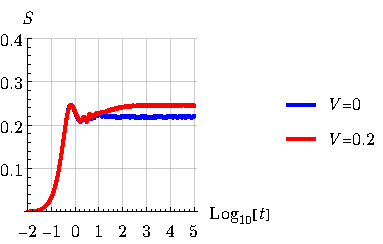
\includegraphics[align=c]{imgs/S_FV1.pdf}
    \hspace{10 mm} 
    \addletter{50}{b} \hspace{2 mm} 
    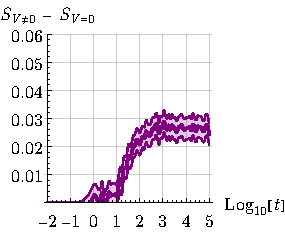
\includegraphics[align=c]{imgs/S_FV2.pdf}
    \caption{a) Entanglement growth. b) The same data but with subtracted values.}
    %\label{fig:}
\end{figure}

Lorem ipsum dolor sit amet, consectetur adipisicing elit, sed do eiusmod
tempor incididunt ut labore et dolore magna aliqua. Ut enim ad minim veniam,
quis nostrud exercitation ullamco laboris nisi ut aliquip ex ea commodo
consequat. Duis aute irure dolor in reprehenderit in voluptate velit esse
cillum dolore eu fugiat nulla pariatur. Excepteur sint occaecat cupidatat non
proident, sunt in culpa qui officia deserunt mollit anim id est laborum.


\begin{figure}[h]
    \centering
    \addletter{150}{a} 
    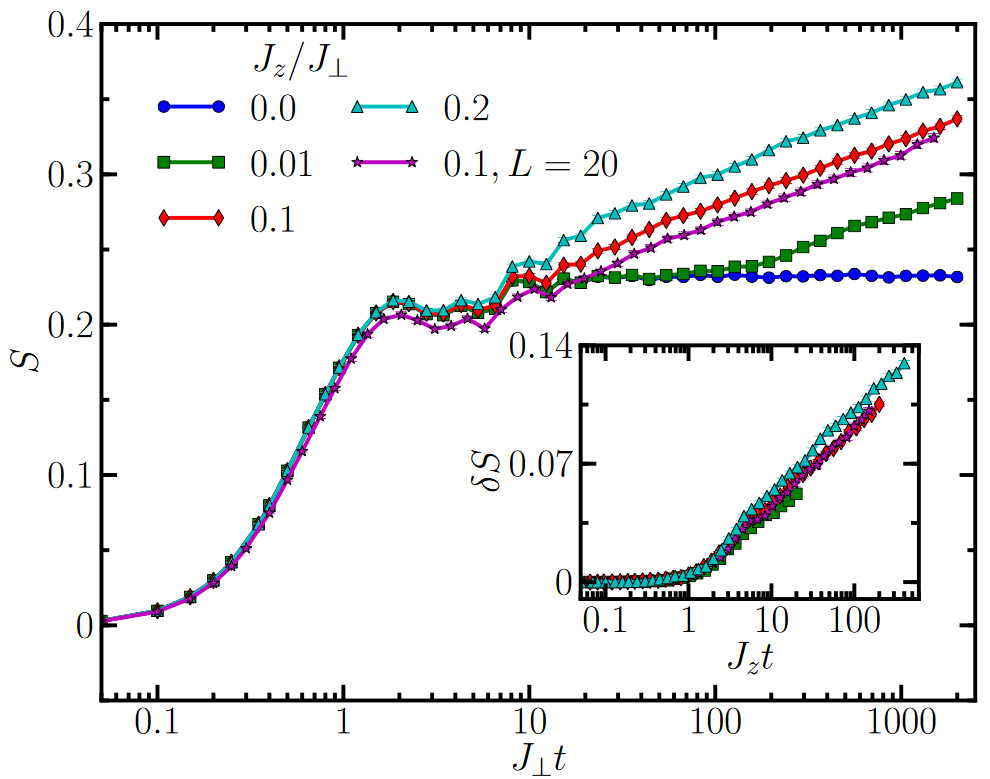
\includegraphics[width=0.4\textwidth]{imgs/S_FV_12a.png}
    \hspace{10 mm} 
    \addletter{150}{b} 
    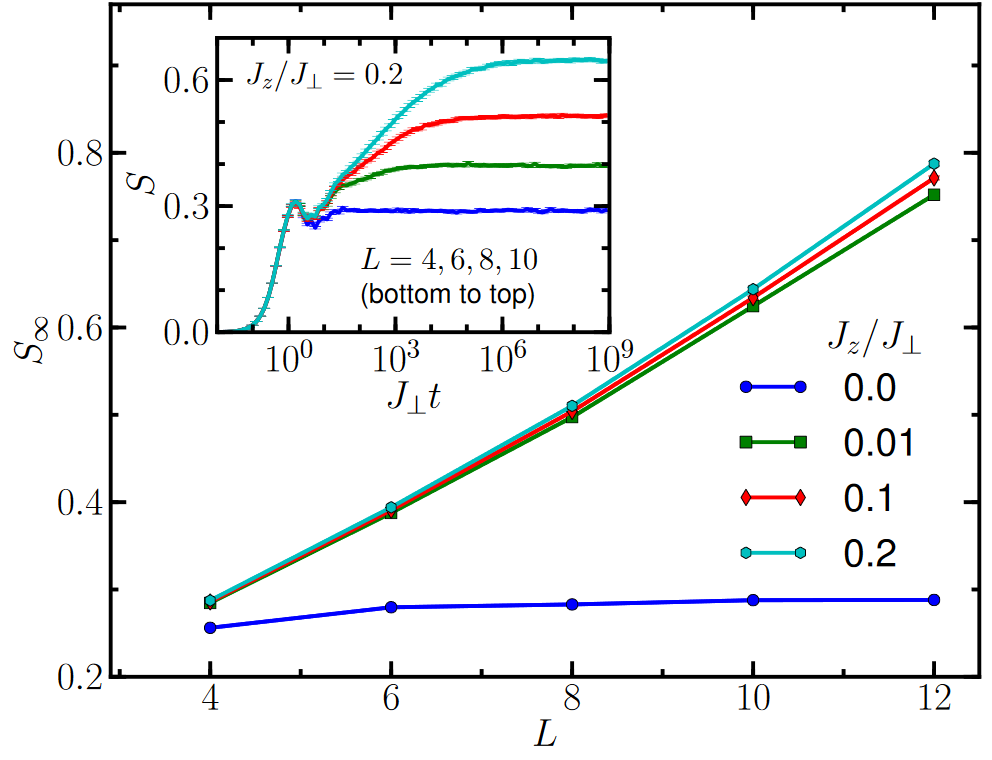
\includegraphics[width=0.4\textwidth]{imgs/S_FV_12b.png}
    \caption{a) Entanglement growth. b) Saturation values of the entanglement entropy as a function of $L$}
    %\label{fig:}
\end{figure}
